\section{Simulations Analyses}
\label{sec:simulations}

%\subsection{Simulation Setup}
In this section, we simulate the game between the attacker and the victim mining pool and study the effectiveness of introducing AWRS against FAW attack.
$\beta$ = 0.24 (which value is derived from the real-world Bitcoin mining and corresponds to the largest pool cap in Bitcoin), $c$ = 0.5 (equal probabilities for the FAW attacker to win and lose the forking race), and $\Gamma = \Gamma_{\mbox{BE}}$ %\textbf{=??? SYC!!!: What is the value of Gamma-BE? Fill in this gap.}  
if the mining pool enables AWRS for protection (as discussed in Section~\ref{sec:theoretical_analyses}), unless otherwise stated in the simulations analyses.
Also, $0 \leq \alpha+\beta \leq 1$ by definition of $\alpha$ and $\beta$.
The results shared in this section holds true in general, i.e., while varying the aforementioned parameters.
%0 < $ $\alpha$ $+$ $\beta$ $ \leq 1$ (when only the attacker and victim pool comprises of the whole bitcoin network) and $ 0 < $ $\alpha$ $+$ $\beta$ $ < 1$ (when there are one or more other mining pools or, miners in the Bitcoin network).
%$\hat{\tau}$ is first calculated using Equation ~\ref{eqn:optimal_tau_faw} and then, the obtained $\hat{\tau}$ is used in ~\ref{eqn:reward_faw} to calculate the reward of a FAW attacker. The reward of a BWH attacker can also be calculated from ~\ref{eqn:reward_faw} by setting c = 0. When the defense mechanism AWRS is used, the reward of a FAW attacker becomes ~\ref{eqn:reward_awrs}. $\hat{\tau}$ for AWSR is calculated by following the same process to find $\hat{\tau}$ from Equation ~\ref{eqn:optimal_tau_faw} for FAW. $\tau_{\mbox{BE}}$ for FAW and AWSR is calculated from the condition reward = $\alpha$,
%where the reward is from Equation ~\ref{eqn:reward_faw} and ~\ref{eqn:reward_awrs} respectively. We have calculated $\Gamma_{\mbox{BE}}$ from Equation ~\ref{eqn:Gamma_BE_tau0}.


%\subsection{Simulation Result}

%Considering the FAW attack in the mining pool as a game, the attacker’s strategy is to maximize his reward using less resource and the pool manager’s strategy is to distribute the earned reward among the miners in the pool according to their computational power. In fact, this is a zero-sum game, where the gain or loss of the attacker will directly affect the gain or loss of the miners in the pool and vice versa. Since, the miners are opportunistic, reward variance is the sole deciding factor for them to join or leave a mining pool.

%The reward maximization of the FAW attacker depends on the computational power of the attacker ($\alpha$), size of the victim pool ($\beta$), the amount of mining power used as infiltration mining ($\tau$) and probability that an attacker’s FPoW through infiltration mining will be selected as main chain (c). However, the attacker can always earn more reward than honest mining regardless of the value of c and the size of the victim pool, $\beta$ \cite{b4}. On the other hand, the reward of the attacker is always an increasing function of the computational power of the attacker and the size of the victim pool, given that the proper $\tau$ is chosen. Considering this, it is always beneficial for the attacker to attack the large pool, as the size of the pool increases, the reward also increases. The reward of the attacker is also an increasing function of c.

%However, this is not the case for infiltration mining power, $\tau$. If $\tau$ increases, then the reward of the attacker will begin to increase or, remain constant up to a certain value of $\tau$ and after that it will begin to decrease. Therefore, it is important for the attacker to calculate $\hat{\tau}$, for which the reward of the attacker will be maximized. Since the FAW attack is always more profitable than honest mining, the attacker will want to use more of his mining power as $\hat{\tau}$ to maximize his reward. Therefore, the attacker will target more powerful victim pool, as it will let him the chance of using more $\hat{\tau}$. However, this is valid for the value of c up to 0.76.

%The reward of the attacker in five different cases such as Honest, FAW, 51\% attack, BWH and AWRS are shown in Fig. \ref{alphavsreward}. It shows that the reward of the FAW attacker is greater than BWH attacker.The difference of reward between BWH and FAW attacker increases as $\alpha$ increases. On the other hand, the reward of the attacker according to our proposed AWRS is always equal to honest mining. Thus, the pool manager can make the attacker’s optimal strategy is to follow honest mining by adopting AWRS.
Fig. \ref{alphavsreward} studies the attacker's reward performance using different strategies while varying the attacker's computational power capability $\alpha$.
When AWRS is disabled, FAW attack outperforms BWH attack and Honest mining.
A 51\% attacker also has the complete control over the reward if it is capable of launching the 51\% attack, i.e., have the majority of the computational power of the network;
the attacker can revoke any blocks that has been mined by others since it controls more power than the rest of the network and can produce a longer chain (forcing the protocol-compliant miners to accept the attacker's chain).
If AWRS is enabled, %using $\Gamma_{\mbox{BE}}$ in Equation~\ref{eqn:Gamma_BE}
then the attacker's performance becomes that of the Honest mining
and there are no incentives for launching FAW or BWH attacks.


\begin{figure}[t]
\centering
\subcaptionbox{Attacker's reward\\with respect to $\alpha$ %{Reward of the attacker \\ (Honest, FAW, 51\%, \\ BWH, AWRS)
\label{alphavsreward}}{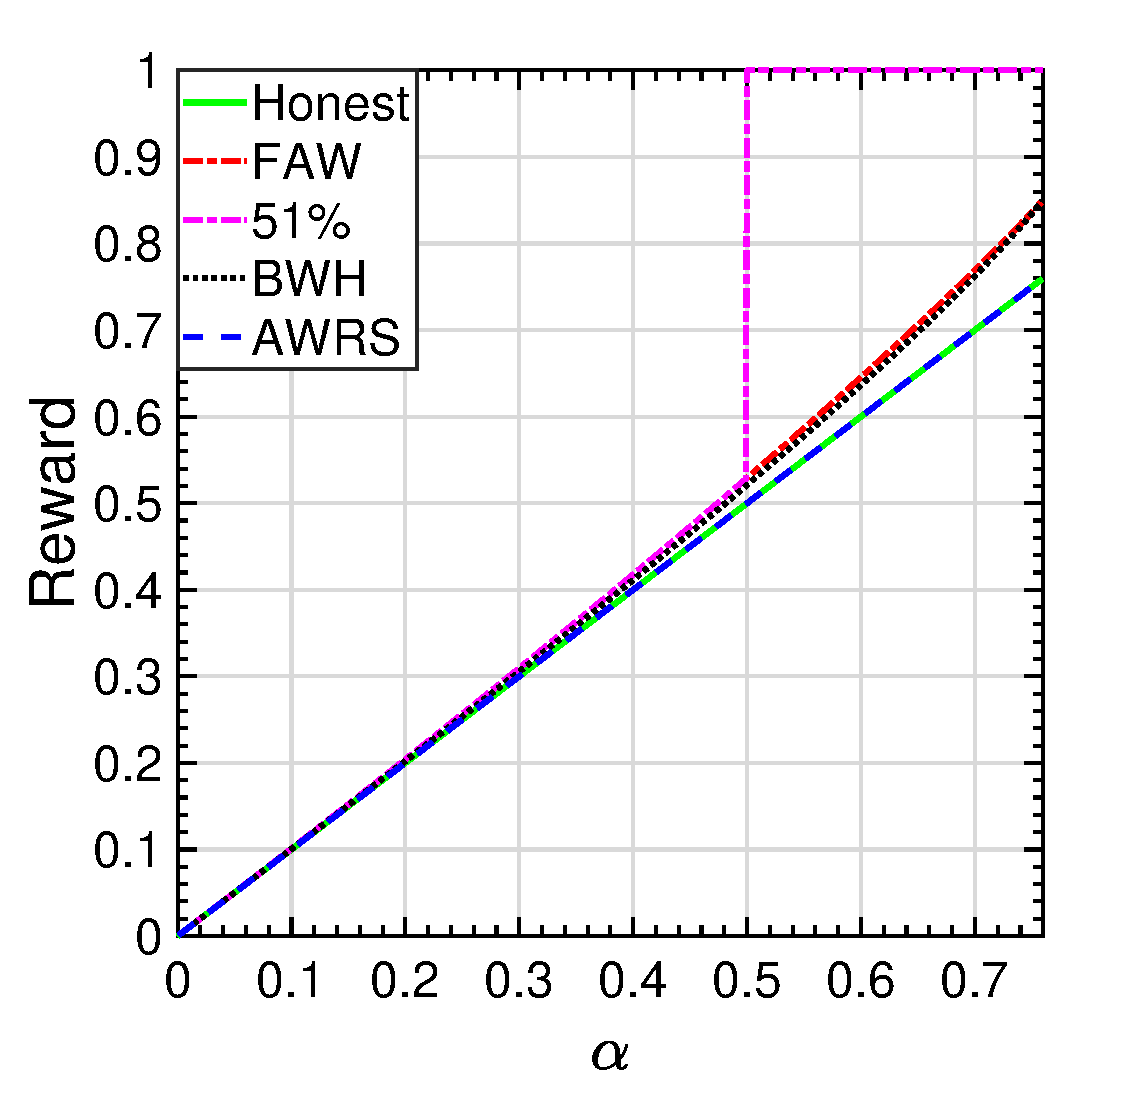
\includegraphics[width=.33\textwidth,height=3cm]{graphics/alphavsreward}}\hfill
\subcaptionbox{$\tau_{\mbox{BE}}$ and $\hat{\tau}$ with\\and without AWRS %Comparison of \\ $\tau_{\mbox{BE}}$ and $\hat{\tau}$ in FAW \\ and AWRS
\label{optimalbreakevenalpha}}{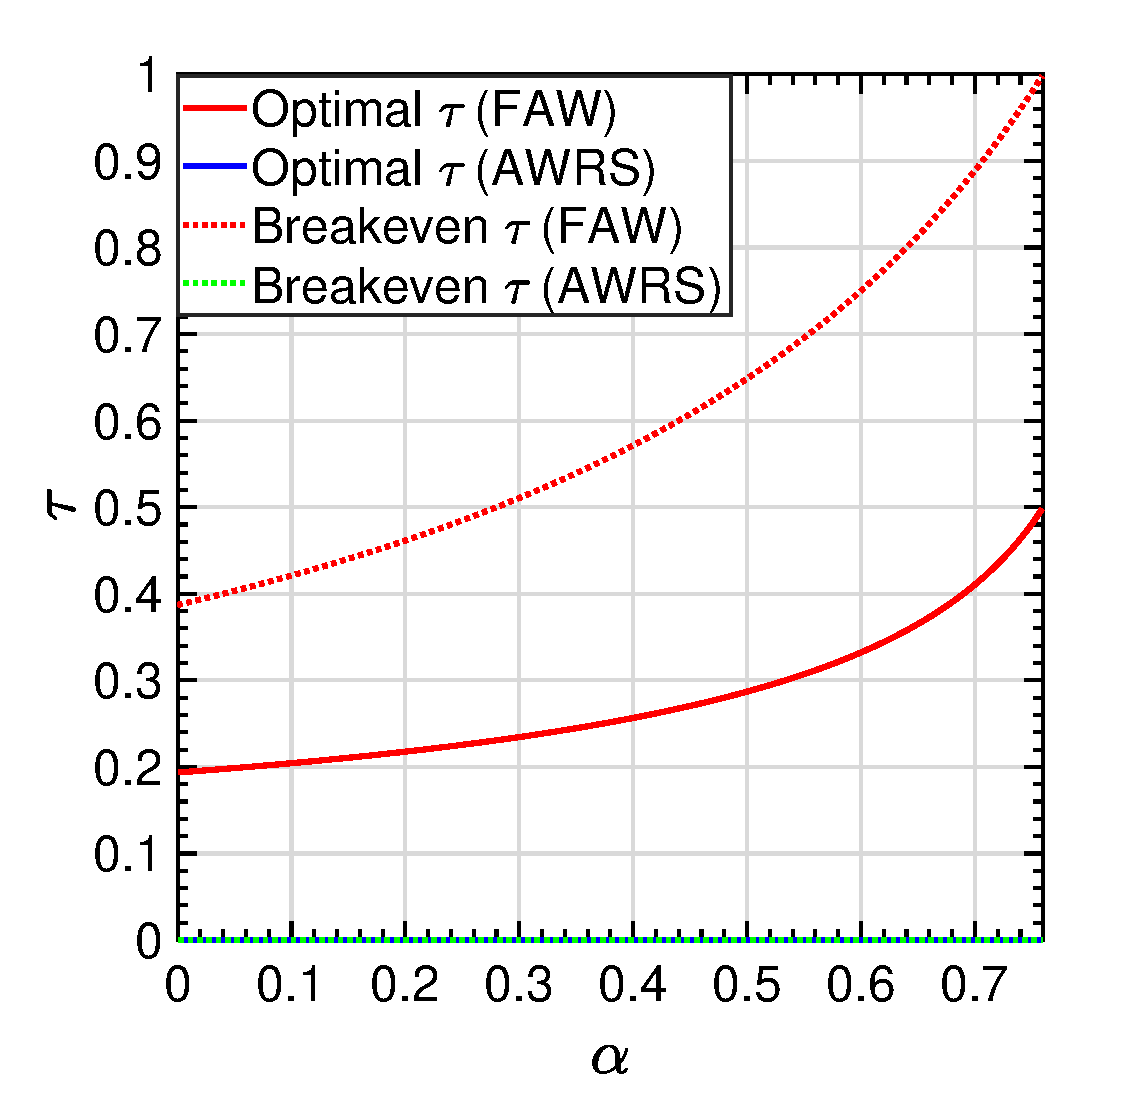
\includegraphics[width=.33\textwidth,height=3cm]{graphics/optimalbreakevenalpha}}\hfill
\subcaptionbox{$\Gamma_{\mbox{BE}}$ with respect to $\alpha$ %{Relation of  $\Gamma_{\mbox{BE}}$ with  $\alpha$
\label{alphavsGammabe}}{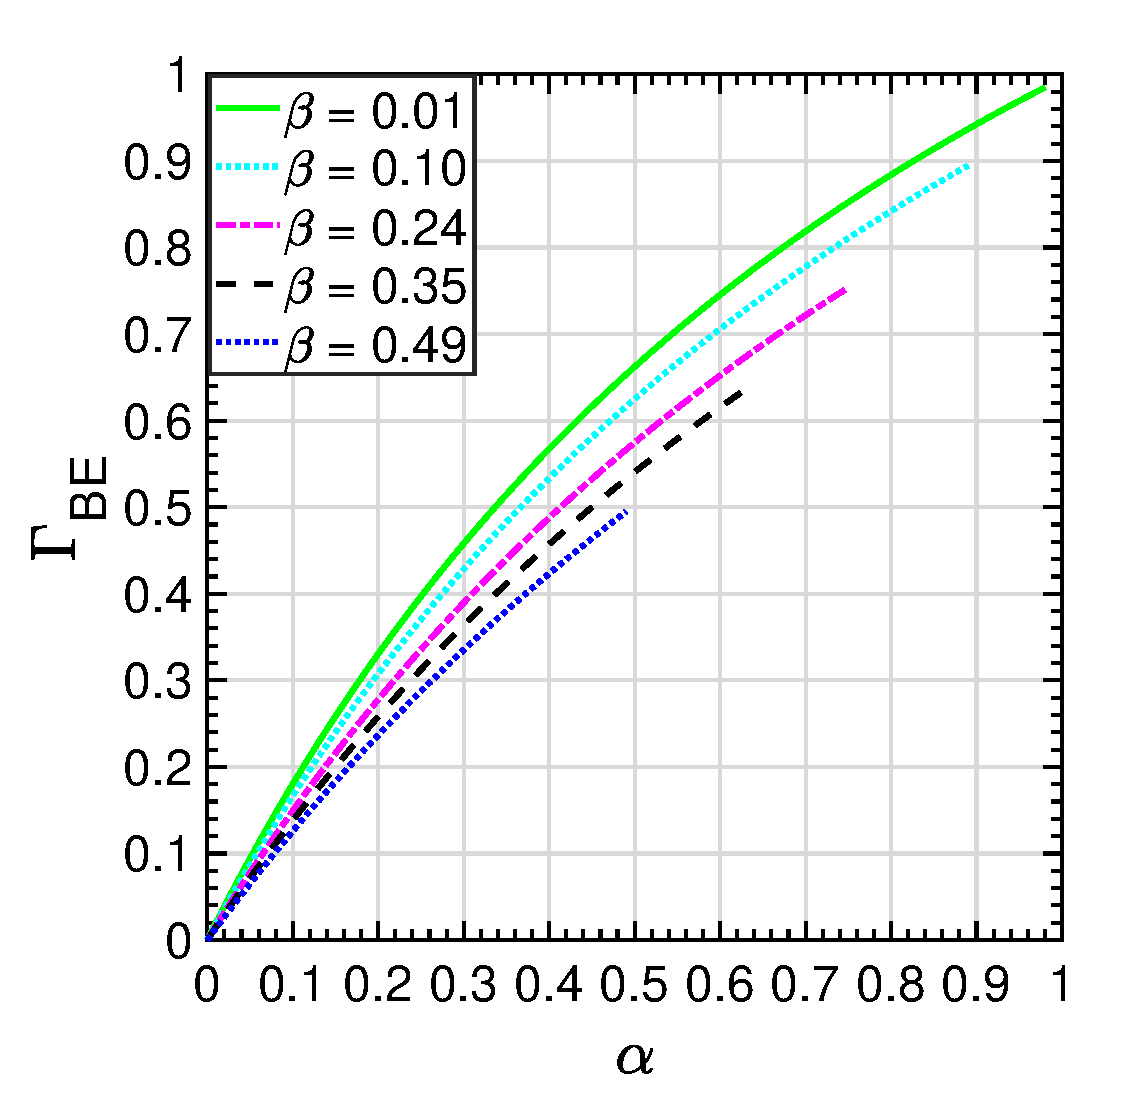
\includegraphics[width=.33\textwidth,height=3cm]{graphics/alphavsGammabe}}\\
\caption{Simulations analyses results} %of AWRS}
\label{fig:AWRS}
\end{figure}

We study the attacker's $\tau$ control between the attacker's main pool and the victim pool, i.e., $0 \leq \tau \leq 1$ where the larger the $\tau$ the greater the infiltration power on the victim pool.
If the victim pool does not enable AWRS, both the $\hat{\tau}$ (discussed in Section~\ref{subsec:faw_attack}) and the $\tau_{\mbox{BE}}$ (yielding $R_{\mbox{FAW}} = \alpha$, i.e., the FAW attack has the same reward as the honest mining) is positive and grows with the attacker's computational capability $\alpha$.
In contrast, with AWRS enabled, the $\hat{\tau}$ and the $\tau_{\mbox{BE}}$ become zero
and the attacker's optimal strategy is not to use any power on the infiltration of the victim pool,
spending all its power on the honest-mining main pool.
%The pool manager’s optimal strategy will be to distribute the reward in such a way that the reward of the attacker will be equal to the honest miner. Therefore, the pool manager will want to keep $\hat{\tau}$ of the attacker close to zero. According to Fig. \ref{optimalbreakevenalpha}, in case of FAW, the more powerful the attacker, the more he can use his optimal infiltration mining power. So, the honest miners in the mining pool will loose more money as the $\alpha$ increases. Also, the $\tau_{\mbox{BE}}$ value is always greater than $\hat{\tau}$ and the difference is very high. Therefore, if the attacker chooses his $\tau$ value less than $\tau_{\mbox{BE}}$, his reward will be always more than honest mining. Fig. \ref{optimalbreakevenalpha} shows that if the pool manager adopts AWRS and use $\Gamma_{\mbox{BE}}$ with $\tau$=0, then $\hat{\tau}$ of the attacker decreases so significantly compared to FAW that it will be incentivized for the attacker to follow honest mining strategy. There is a reason behind using $\tau$=0 for the calculation of $\Gamma_{\mbox{BE}}$. Because for any other value of $\tau$, the reward of the attacker is always greater than $\tau$=0. Therefore, the pool manager does not need to worry about the $\tau$ value of the attacker.

Fig. \ref{alphavsGammabe} studies the dependency of $\Gamma_{\mbox{BE}}$ (which is the lower bound on the pool's reward portion to the block submitter for AWRS to deprive the incentives of the FAW attack) on the attacker's computational power ($\alpha$) and the victim pool's computational power ($\beta$).
As $\alpha$ grows, the bound in $\Gamma_{\mbox{BE}}$ grows (in fact, $\Gamma_{\mbox{BE}}\geq \alpha$ in general) and, as $\beta$ grows, $\Gamma_{\mbox{BE}}$ reduces (providing greater flexibility in $\Gamma$ control in AWRS).
%On the other hand, there is a relation between $\Gamma_{\mbox{BE}}$ and the computational power of the attacker. The threshold value of $\Gamma_{\mbox{BE}}$ is always greater than $\alpha$. That means, the more powerful attacker attacks a mining pool, the more will be the value of $\Gamma_{\mbox{BE}}$. Therefore, the more powerful attacker attacks a mining pool, the special reward to the block submitter will increase to make the reward of the attacker equal to honest mining. On the contrary, the relation between $\Gamma_{\mbox{BE}}$ and the size of the victim pool is inversely proportional. The bigger the size of the victim pool, the less becomes the value of $\Gamma_{\mbox{BE}}$. These relatioships are shown in Fig. \ref{alphavsGammabe}. In Fig. \ref{alphavsGammabe}, the value of  c = 0.5, but for other values of c, this is also true.
